% Created 2019-03-13 Wed 19:58
% Intended LaTeX compiler: pdflatex
\documentclass[english,odsaz]{fitthesis}
\renewcommand\title[1]{}
%%% Local Variables:
%%% mode: latex
%%% TeX-master: "projekt.org"
%%% End:

\projectinfo{
  project={BP},
  year={2019},
  date=\today,
  title.cs={Název práce},
  title.en={Thesis title},
  %title.length={14.5cm},
  author.name={Jakub},
  author.surname={Zárybnický},
  department={UITS},
  faculty={FIT},
  supervisor.name={Ondřej},
  supervisor.surname={Lengál},
  supervisor.title.p={Ing.},
  supervisor.title.a={Ph.D.},
  keywords.cs={Sem budou zapsána jednotlivá klíčová slova v českém (slovenském) jazyce, oddělená čárkami.},
  keywords.en={Sem budou zapsána jednotlivá klíčová slova v anglickém jazyce, oddělená čárkami.},
  abstract.cs={Do tohoto odstavce bude zapsán výtah (abstrakt) práce v českém (slovenském) jazyce.},
  abstract.en={Do tohoto odstavce bude zapsán výtah (abstrakt) práce v anglickém jazyce.},
  declaration={Hereby I declare that this bachelor's thesis was prepared as an
    original author’s work under the supervision of Ing. Ondřej Lengál,
    Ph.D. All the relevant information sources used during preparation of this
    thesis are properly cited and included in the list of references.},
  %acknowledgment={Here it is possible to express thanks to the supervisor and
  %  to the people which provided professional help (external submitter, consultant, etc.).},
  extendedabstract={Do tohoto odstavce bude zapsán rozšířený abstrakt práce v
    českém jazyce, bude mít rozsah 2 až 6 normostran a bude obsahovat úvod,
    popis vlastního řešení a shrnutí a zhodnocení dosažených výsledků.},
}

\usepackage{minted}
\usepackage[figure,table]{totalcount}
\date{\today}
\title{}
\hypersetup{
 pdfauthor={},
 pdftitle={},
 pdfkeywords={},
 pdfsubject={},
 pdfcreator={Emacs 26.1 (Org mode 9.1.9)}, 
 pdflang={English}}
\begin{document}

% * (front matter)                                              :ignoreheading:
\maketitle
\setlength{\parskip}{0pt}
{\hypersetup{hidelinks}\tableofcontents}
\iftotalfigures\listoffigures\fi
\iftotaltables\listoftables\fi
\iftwoside\cleardoublepage\fi
\setlength{\parskip}{0.5\bigskipamount}

\chapter{Introduction}
\label{sec:org270e8c8}
[TODO: reword Intro\&Tech - more flowing language]

Let's imagine we want to create a new e-shop, with all the conveniences that
customers are nowadays used to - [TODO: \ldots{}], a notification when the order is
ready, and ideally an offline-available overview of the order for when the user
is picking it up. What would be the easiest way to implement such a service? If
we want to show something offline, we need a mobile application, the same for
notifications. But [TODO: research about mobile engagement] and downloading a
mobile application means another dozen megabytes.

This is what the new trend of Progressive Web Applications (PWAs) is trying to
solve. Fast - no need to wait for page reloads - and reliable - service workers help
overcome problems with unreliable internet, both for page load by caching the
app itself and in-app caching of app-specific data, and for background sync of
user-modified data.

My language of choice is Haskell though, for both frontend and backend
development, and while writing Haskell applications for the browser is possible,
creating a Progressive Web Application requires more than just the ability to
manipulate the DOM. That is what this work is about - filling in the gaps and
creating all the prerequisites for writing Progressive Web Applications in
Haskell. We will start by identifying exactly what is lacking in the Haskell
ecosystem, and designing and implementing those missing pieces. Afterwards, we
will walk through the process of creating a PWA from prototype to production and
see what else could be made easier and more straightforward as a follow-up to
this work.

\section{Related work}
\label{sec:org2d34576}
While using Haskell in the browser is not a common choice, the adoption is
steadily growing. Any work in this area is relatively recent though, as the
Haskell-to-JavaScript compiler, GHCJS, has only been in development since 2010
\cite{ghcjs}, with a production-ready version in 2013 \cite{ghcjs-luite}. Academic
work on GHCJS or related projects is sparse, but there are several commercially
sponsored projects - to name a few, Reflex and Obelisk from Obsidian Systems
\cite{obsidian}, Asterius from Tweag, and many learning materials from QFPL
\cite{qfpl}.

\chapter{Technologies}
\label{sec:org3077323}
We will first have a more detailed look at the above-mentioned technologies, at
what the term Progressive Web Application means and why would one want to use
Haskell when creating browser applications.

\section{Progressive Web Application}
\label{sec:org5b11da4}
'Progressive Web Application' is a term that covers several relatively new
technologies. It is the continuation of the general trend of expanding the
capabilities of browser applications and closing the gap between them and native
mobile applications. While many of these technologies apply also on desktop, the
main target audience is mobile - [TODO: some statistics].

The technologies are:
\begin{itemize}
\item Web App Manifest - a specification for the centralized location of application
metadata - its name, icons, display mode, \ldots{}
\item Service Workers - 'a scriptable network proxy' \cite{mdn_svcwrk}. The
technology that takes care of offline-availability, push notifications, and
background synchronization.
\item IndexedDB - a storage location that is accessible from the browser as well as
the service worker, it allows background sync to work with the application
state directly
\item Web Platform APIs - a set of APIs that expose capabilities of the underlying
system - examples include geolocation or
audio/video capture \cite{what_web_can_do}
\end{itemize}

What is a Progressive Web Applications exactly is defined by a checklist created
by Google \cite{pwa_checklist}. It describes two levels of PWAs, a 'Baseline PWA'
and an 'Exemplary PWA'. The main defining characteristics of a Baseline PWA are:
served over HTTPS, responsive design, all URLs available even while offline, and
non-blocking page transitions. While there are more requirements for an
Exemplary PWA, these are the most important ones.

Some more notable PWAs are: Twitter \cite{twitter}, Uber \cite{uber}, or Flipkart
\cite{flipkart}.

\section{Haskell}
\label{sec:org7c33a66}
\begin{listing}[htbp]
\begin{minted}[,frame=single]{haskell}
type HackageAPI =
  "users" :> Get '[JSON] [User] :<|>
  "user" :> Capture "login" Login :> Get '[JSON] User :<|>
  "packages" :> Get '[JSON] [Package]

getUsers :: Handler [User]
getUser :: Login -> Handler User
getPackages :: Handler [Package]

server :: Server HackageApi
server = getUsers :<|> getUser :<|> getPackages

getUsers :<|> getUser :<|> getPackages =
  client @HackageApi "http://hackage.haskell.org"
\end{minted}
\caption{An example of a web server in Haskell}
\end{listing}

The programming language Haskell is a rather old one. Despite spreading into the
industry only recently, it has been in development since 1990
\cite{haskell_history}. It started out as government research project, a common
base for programming language research. It has served as such, and in fact it
still is the target of active research - some more prominent projects are
'Dependent Haskell' \cite{eisenberg2016dependent} and 'Linear Haskell'
\cite{bernardy2017linear}.

[TODO: reword] Haskell is described as a ``statically typed, purely functional
programming language with type inference and lazy evaluation''
\cite{jones2003haskell}. It is a language in which its expressive type system
enables precise control over TODO: expressive types, dialog with the compiler,
types encoding effects, citation for ``If it compiles, it works''.

[TODO: reword] Why Haskell? It is a strongly typed language, which helps ensure
correctness and prevent undefined behaviors - but it is less verbose and more
expressive than Java and other languages a developer would imagine as 'strongly
typed'. Haskell is one of the many languages capable of running in the browser -
not directly, but by compiling down to JavaScript. Another technology that
enables languages to run in the browser is WebAssembly, an alternative assembly
language and a runtime designed specifically for the Web. Compiling Haskell for
the Web via WebAssembly is almost doable, there are two active projects creating
a Haskell compiler backend - WebGHC \cite{webghc} and Asterius \cite{asterius}.

Compile-to-JavaScript languages are not as rare as it may sound. While languages
not based on JavaScript itself are not exactly common, web developers have been
using JavaScript compilers for a long time - CoffeeScript is rather popular
language announced in 2010 \cite{coffeescript}, and developers wanting to use new
ECMAScript 6 or 7 features (now supported in most browsers) also had no choice
but to use compilers \cite{babel}.

It is a language that enables its users to write reliable software by
eliminating entire classes of programming errors \cite{Nanz_2015}. The errors that
remain even after the program successfully compiles are usually logic or
conceptual errors.

While Haskell is not a language commonly associated with frontend development,
it is one of the many languages with the ability to use JavaScript as the
compilation target, instead of plain assembly or LLVM. In fact, such languages
have now become quite common in frontend development, as is exemplified by the
rapid rise of TypeScript, a superset of ECMAScript 6 \cite{typescript}, or Elm, a
framework with its own language based on Haskell \cite{czaplicki2012elm}.

Of the many reasons for selecting a language other than JavaScript for frontend
development, one of the more notable ones is the ability to share code between
the server and its client in the case they are written in the same
language. This is the basic idea of the framework Meteor \cite{meteor}, and in
fact the ability to run 'isomorphic code' - the same code on the client and the
server both - is its main marketing point.

\section{Nix}
\label{sec:orgbfbba00}
\begin{listing}[htbp]
\begin{minted}[,frame=single]{nix}
{ stdenv, fetchurl, perl }:

stdenv.mkDerivation {
  name = "hello-2.1.1";
  builder = ./builder.sh;
  src = fetchurl {
    url = ftp://ftp.nluug.nl/pub/gnu/hello/hello-2.1.1.tar.gz;
    sha256 = "1md7jsfd8pa45z73bz1kszpp01yw6x5ljkjk2hx7wl800any6465";
  };
  inherit perl;
}
\end{minted}
\caption{An example Nix derivation of GNU hello}
\end{listing}

One technology not yet mentioned, but upon which stands the entire build system
used in this work from compiling to deploying, is Nix. Nix
\cite{dolstra2006purely} is a package manager with focus on reproducibility and
isolation. It is described as a purely functional package manager, where every
package is built by a function without side-effects, with the result being
immutable. Nix also ensures the exact versions of dependencies are used even
during runtime - all the way up to \texttt{libc}.

Nix is a declarative build tool, similar in purpose to Make and in philosophy to
Haskell. There are other tools built on top of Nix though, the most interesting
being NixOS, a declarative operating system, and NixOps, a cloud deployment tool
\cite{dolstra2008nixos}. Nix shines at cross-compilation, which is the main we
will use it in this work - compiling to JavaScript or Android/iOS is trivial
after the initial setup.

Nix is another rather old technology under active development since 2004 after
Eelco Dolstra introduced this idea in his academic work
\cite{dolstra2006purely}. One package consists of a closure of all of its runtime
dependencies, so even packages using different versions of dynamically linked
libraries or even libc can coexist on the same machine. Adding atomic
deployments and rollbacks is then quite easy, as a user environment only
consists of symbolic links to the read-only Nix store, which is useful for NixOS
or NixOps.

\chapter{Research}
\label{sec:org71399d4}
As this work does not live in a vacuum, we also need to consider commonly used
Web frameworks and platforms and decide what features to implement in. We will
first walk through the features that frameworks today implement, describe them
and define the relevant terms. Afterwards, we will have a brief look at the
specifics of the JavaScript ecosystem - the most common language in Web
development - and the of Haskell, my language of choice, and try to find the
places where Haskell is lagging behind and especially the features that we will
need to fill in in this work.

\section{Features of Web frameworks}
\label{sec:org89fc9a8}
The basis of a web framework is the \textbf{UI toolkit}, which defines the structure,
architecture and paradigm of the rest of the application. I am intentionally
using the now-uncommon term 'toolkit', as the UI frameworks we will see vary in
their scope - e.g. React is just a library with a small API, whereas Angular
provides a quite opinionated platform. Individual frameworks are quite
disparate, with large differences in the size of their community, maturity,
developer friendliness and the breadth of features or available libraries.

Frameworks usually have one defining feature they are built around (virtual DOM
for React or event streams for Angular), but there are many other concerns that
a framework needs to take care of. \textbf{Templating} is one of the essential ones. It
is a way of composing the HTML that makes up an application which also usually
includes some 'view logic' and variable interpolation. In some frameworks the
whole program is a template (purely functional React), some have templates in
separate files and pre-compile them during the build process or even in the
browser (Angular). Templates may also contain CSS as well - see the new
CSS-in-JS trend.

The second defining feature of frameworks is \textbf{state management}. This rather vague
concept may include receiving input from the user, displaying the state back to
the user, communicating with APIs and caching the responses, etc. While state
management is simple at a small scale, there are many problems that appear only
in larger applications with several developers. Some approaches include: a
'single source of the truth' and immutable data (Redux), local state in
hierarchical components (Angular), or unidirectional data flow with several
entity stores (Flux).

Another must-have feature of a framework is \textbf{routing}, which means manipulating
the displayed URL using the History API, and changing it to reflect the
application state and vice-versa. It also includes switching the application to
the correct state on start-up. While the router is usually a rather small
component, it is fundamental to the application in the same way the previous two
items are.

A component where frameworks differ a lot is a \textbf{forms} system. There are a few
layers of abstraction at which a framework can decide to implement forms,
starting at raw DOM manipulation, going on to data containers with validation
but manual rendering, all the way up to form builders using domain-specific
languages. The topic of 'forms' includes rendering a form and its data,
accepting data from the user and validating it, and sometimes even submitting it
to an API.

There are other features that a framework can provide - authentication,
standardized UI components, and others - but frameworks usually leave these to
third party libraries. There is one more topic I would like to mention that is
usually too broad to cover in the core of a framework, but important to consider
when developing an application. \textbf{Accessibility} is an area concerned with removing
barriers that would prevent any user from using a website. It has many parts to
it - while the focus is making websites accessible to screen-readers, it also
includes supporting other modes of interaction, like keyboard-only
interaction. Shortening \textbf{load times} on slow connections also makes a website
accessible in parts of the world with slower Internet connections, and
supporting \textbf{internationalization} removes language and cultural barriers.

Accessibility is something that requires framework support on several
levels. Making a site accessible requires considerations during both design
(e.g. high color contrast) and implementation (semantic elements and ARIA
attributes), and that is usually left up to application code and accessibility
checklists, with the exception of some specialized components like keyboard
focus managers. There are however tools like aXe-core that check how accessible
a finished framework is, and these can be integrated into the build process.

\textbf{Internationalization} is somewhat easier to support in a framework, as it does
include so many cross-cutting concerns. At the most basic level, it means simple
string translations, perhaps with pluralization and word order. Going further,
it may also mean supporting RTL scripts, different date/time formats, currency,
or time zones.

As for \textbf{load times}, there are many techniques frameworks use to speed up the
initial load of an application. We can talk about the first load, which can be
sped up by compressing assets (CSS, fonts, fonts or scripts) and removing
redundant ones, or by preparing some HTML that can be displayed to the user
while the rest of the application is loading to increase the perceived
speed. After the first load, the browser has some of the application's assets
cached, so loading will be faster. One of the requirements of a PWA is using the
Service Worker for instantaneous loading after the first load.

There are two patterns of preparing the HTML that is shown while the rest of the
application is loading - so called \textbf{prerendering}. One is called 'app shell',
which is a simple static HTML file that contains the basic structure of the
application's layout. The other is 'server-side rendering', and it is a somewhat
more advanced technique where the entire contents of the requested URI is
rendered on the server including the data of the first page, and the browser
part of the application takes over only afterwards, without the need to fetch
any more data. There is another variant of 'server-side rendering' called the
'JAM stack' pattern \cite{jamstack}, where after application state changes, the
HTML of the entire application, of all application URLs is rendered all at once
and saved so that the server does not need to render the HTML for every
request. These techniques are usually part of a framework's \textbf{supporting tools},
about which we will talk now.

Developers from different ecosystems have wildly varying expectations on their
tools. A Python developer might expect just a text editor and an interpreter,
whereas a JVM or .NET developer might not be satisfied with anything less than a
full-featured IDE. We will start with the essentials, with \textbf{build
tools}. Nowadays, even the simplest JavaScript application usually uses a build
step that packages all its source code and styles into a single bundle for
faster loading. A framework's tool-chain may range from a set of conventions on
how to use the compiler that might get formalized in a Makefile, through a CLI
tool that takes care of building, testing and perhaps even deploying the
application, to the way of the IDE, where any build variant is just a few clicks
away.

\textbf{Debugging tools} are the next area. After building an application, trying it out,
and finding an error, these tools help in finding the error. There are generic
language-specific tools - a stepping debugger is a typical example - and there
are also framework-specific tools, like an explorer of the component hierarchy
(React) or a time-traveling debugger (Redux). In the web world, all modern
browsers provide basic debugging tools inside the 'DevTools' - a stepping
debugger and a profiler. Some frameworks build on that and provide an extension
to DevTools that interacts with the application in the current window, some
provide debugging tools integrated into the application itself.

When building or maintaining a large application with several developers, it is
necessary to ensure good practices in all steps of the development
process. There are two general categories in \textbf{quality assurance} tools - testing
(dynamic analysis) tools and static analysis tools. In the commonly used
variants, tests are used either as an aid while writing code (test-driven
development), or to prevent regressions in functionality (continuous integration
using unit tests and end-to-end tests). Static analysis tools are, in the
general practice, used to ensure a consistent code style and prevent some
categories of errors ('linters'). Frameworks commonly provide pre-configured
sets of tools of both types. If necessary - e.g. in integration testing where
the burden of set up is bigger - they also provide utility libraries to ease the
initial set up. Some frameworks also use uncommon types of tests like 'marble
tests' used in functional reactive programming systems.

\textbf{Editor integration} is also important in some ecosystems. This includes common
features of Integrated Development Environments like auto-completion or
refactoring tools. Recently the Language Server Protocol (LSP) \cite{lsp} project
played a big role in allowing editors to support a wide variety of languages by
implementing just an LSP client and being able to communicate with any
language-specific language server. There are some parts of editor support that
can be framework-specific like supporting an embedded domain-specific language
or integrating framework-specific debugging tools.

While we were talking about Web frameworks so far, some of them support not only
running inside the browser but also being packaged as a \textbf{mobile app} for Android
or iOS, or as a \textbf{native desktop application} for the many desktop operating
systems. For mobile support, frameworks often provide wrappers around Apache
Cordova, which is a thin wrapper around a regular website exposing some extra
capabilities of the device. Some, however, go even further and support fully
native mobile interfaces controlled by JavaScript, like React Native. The
situation is similar for desktop support, just with Electron used as the base
instead of Cordova. The main benefits of packaging a Web application instead
just running it inside a browser are performance (they are usually faster to
load and to use), access to device-specific capabilities (direct access to the
file system), or branding.

The last point in this section is \textbf{code generators}. of which there are two
variants: project skeleton generators, which create all files necessary for a
project to compile and run, and which are provided in a large majority of
frameworks. Then there are component generators, which may include generating a
template, a URL route and its corresponding controller, or an entire subsection
of a website. These are less common but some frameworks also provide them.

\section{JavaScript ecosystem}
\label{sec:org6d33cfc}
Moving on, we will take a quick tour of the JavaScript ecosystem and what the
library ecosystem looks there, following the same general structure as we have
used in the section above.

The most popular \textbf{UI toolkits} in JavaScript are currently Angular \cite{angular}
and React \cite{react}. Vue.js \cite{vuejs} is another, a relatively new but quickly
growing one. Of these, Angular is the framework closest to traditional
frameworks where it tries to provide everything you might need to create an
application. React and Vue are both rather small libraries but with many
supporting tools and libraries that together also create a platform, although
they are much less cohesive than Angular's platform.

There are fundamental architectural differences between them. Angular uses plain
HTML as a base for its templates, and uses explicit event stream manipulation
for its data flow. React uses a functional approach where a component is (de
facto) just a function producing a JavaScript object, in combination with an
event-driven data flow. Vue uses HTML, CSS and JavaScript separately for its
templates, and its data flow is a built-in reactive engine.

The most common complaint about the JavaScript ecosystem in general is that it
is a 'jungle'. There are dozens or hundreds of small libraries doing the same
thing, most however incomplete or unmaintained, with no good way to decide
between them. Frameworks avoid this problem by having a recommended set of
libraries for common use cases. A different but related complaint is called the
'JavaScript fatigue'. The trends change quickly in the JavaScript ecosystem,
libraries come and go each year, a common belief is that if you are not learning
at least one new framework per year, you are missing out on opportunities.

As for the individual frameworks mentioned above: Angular is an integrated
framework that covers many common use cases in the basic platform. To some
though, it is too opinionated, too complex to learn easily, or with too much
abstraction to understand.

React and Vue are rather small libraries which means they are very flexible and
customizable. There are many variants of libraries for each feature a web
application might need, which also means that it is easy to get stuck deciding
on which library to pick out of the many options. There are React and Vue
'distributions', however, that try to avoid this by picking a set of libraries
and build tools that works together well.

As for the topics mentioned in the previous section - routing, forms, build
tools, mobile and desktop applications - most are built into Angular, and for
React and Vue there are dozens of options of third party libraries. In my
investigation, I have not found a weak side to any of them - which is just what
I expected, given that JavaScript is the native language of the Web.

\section{Haskell ecosystem}
\label{sec:orgc30e63d}
Going on to the Haskell ecosystem, we will also walk through it using the
structure from the 'Features' section. There is significant focus on the
semantics of libraries in the Haskell community, e.g. writing down mathematical
laws for the foundational types of a library and using them to prove correctness
of the code, so UI libraries have mostly used Functional Reactive Programming
(FRP) or its derivatives like 'the Elm architecture' \cite{loder2018web} as their
basis, as traditional imperative event-based programming does not fit those
criteria well.

There are five production-ready UI toolkits for the Web that I have found. Of
these five, React-flux and Transient are unmaintained, and Reflex, Miso, and
Concur are actively developed and ready for production use. Each one uses a
conceptually different approach to the problem of browser user interfaces, and
they differ in their maturity and the size of their community as well.

\textbf{Reflex} \cite{reflex} (and Reflex-DOM \cite{reflex-dom}, its DOM bindings) looks like
the most actively maintained and developed one. Reflex is also sponsored by
Obsidian Systems \cite{obsidian} and is the most popular frontend framework in the
Haskell community, so its future seems promising. Reflex follows the traditional
FRP approach with events and behaviors (adding 'dynamics'), and
building a rich combinator library on top of them.

\begin{listing}[htbp]
\begin{minted}[,frame=single]{haskell}
main :: IO ()
main = mainWidget $ display =<< count =<< button "Click me"
\end{minted}
\caption{An example of Reflex code (a counter)}
\end{listing}

\textbf{Miso} \cite{miso} is a re-implementation of the 'Elm architecture' in Haskell,
which means that is uses strictly uni-directional data-flow with a central data
store on the one side, and the view as a pure function that takes the state and
creates a view on the other, where the view can change the state using strictly
defined events. The ecosystem of Miso is not as well developed as Reflex's, and
the overall architecture is very limiting - which I consider a large
disadvantage.

\begin{listing}[htbp]
\begin{minted}[,frame=single]{haskell}
type Model = Int

data Action = AddOne
  deriving Eq

main :: IO ()
main = JSaddle.run 8080 $ startApp App {..}
  where
    initialAction = AddOne
    model  = 0
    subs   = []
    events = defaultEvents
    mountPoint = Nothing

    update AddOne m = noEff (m + 1)

    view x = div_ []
      [ text (ms x)
      , button_ [ onClick AddOne ] [ text "Click Me" ]
      ]
\end{minted}
\caption{An example of Miso code (a counter)}
\end{listing}

\textbf{Concur} \cite{concur} tries to explore a different paradigm by combining 'the best
of' the previous two approaches. The developers have so far been focusing on
exploring how this paradigm fits into browser, desktop or terminal applications,
so it has a quite small range of features. It is a technology I intend to explore
in the future when it is more mature, which however does not seem suitable for a
large application so far, at least compared to its competitors.

\begin{listing}[htbp]
\begin{minted}[,frame=single]{haskell}
main :: IO ()
main = do
  initConcur
  void $ runWidgetInBody $ void $ flip execStateT (0 :: Int) $
    forever $ increment1 <|> displayCount
  where
    increment1 = lift (el_ E.div [] $ button "Click Me") >> modify (+10)
    displayCount = do
      count <- get
      lift $ el_ E.div [] $ text $ show count ++ " clicks"
\end{minted}
\caption{An example of Concur code (a counter)}
\end{listing}

In all of these frameworks, \textbf{templating} is a feature that has been side-stepped
by creating a domain-specific language for HTML mixed with control flow. There
have been attempts at creating a more HTML-like language embedded into Haskell
or external templates, though there is no such project that is both
feature-complete and actively maintained. It is however possible to reuse
existing JavaScript components using the foreign function interface (FFI)
between Haskell and JavaScript, and that it exactly what one of the unmaintained
frameworks did to use React as its backend (react-flux).

\textbf{State management} is where the frameworks differ the most. Miso follows the Elm
architecture strictly with a central data store that can be only changed by
messages from the view, whereas Reflex and Concur are more flexible, allowing
both centralized and component-local state. A common complaint regarding Reflex
is that there is no recommended application architecture - it errs on the
other side of the flexibility vs. best practices spectrum.

As for \textbf{routing}, Miso has routing built into its base library. There are several
gattempts at a routing library in Reflex, though the situation is the same as
with templating libraries. Concur with its small ecosystem does not have routing
at all, it would be necessary to implement form scratch for a production-ready
application.

In \textbf{forms} - and UI components in general - the selection is not good. There
are several components collections for Reflex which use popular CSS frameworks
(Bootstrap, Semantic UI), though each has many missing pieces and they lack
components that need to be re-implemented anew in each application - forms in
particular. Miso and Concur do not have any publicly available UI component
libraries, or at least none that I was able to find.

\textbf{Accessibility} as a whole has not been a focus of Web development in Haskell. It
is possible to reuse JavaScript accessibility testing tools however, though I
have not seen any sort of automated testing done on any of the publicly
available Haskell applications. The only area with continued developer focus is
\textbf{loading speed}, as the size of build artifacts was a problem for a long
time. That has been ameliorated to the level of a common JavaScript application
however, so that is not a critical concern. \textbf{Prerendering} is also supported by
Miso and Reflex, which helps speed up load times as well.

Moving on to the topic of \textbf{build tools}: there are three main options in Haskell -
Cabal v2 \cite{cabal}, Stack \cite{stack}, and Nix. There are also other options -
Snack \cite{snack}, aiming for the best of these three but not yet ready for
production use, or Mafia \cite{mafia}, which is not too popular in the community
at large. Cabal is the original Haskell build tool which gained a bad reputation
for some of its design decisions (the so-called 'Cabal hell'), though most of
them were fixed in 'Cabal v2' which puts it on par with its main competitor,
Stack. Stack tried to bring Haskell closer to other mainstream programming
language by introducing several new features like automatic download of the
selected compiler or a curated subset of the main Haskell package repository,
Stackage. It succeeded in that, becoming the tool of choice for a large part of
the Haskell community in the process. Nix, as mentioned in the previous section,
is a general-purpose build tool and not a Haskell-specific one. It has very good
cross-compilation capabilities, however, which is the reason it is especially
used for frontend Haskell.

Glasgow Haskell Compiler (GHC) is the main Haskell \textbf{compiler} used for the
creation of native binaries. Compilation to JavaScript, as required for frontend
development, is supported by a separate compiler, GHCJS, which uses GHC as a
library. Setting up a GHCJS development environment with Cabal is not a trivial
process and using Stack limits the developer to old GHC versions, so it is Nix
that is usually recommended. When set up correctly, Nix offers almost a
one-click setup, downloading the compiler and all dependencies from a binary
cache or compiling them if unavailable. Reflex especially, in the
reflex-platform \cite{reflex-platform} project, uses the cross-compilation
capabilities of Nix to allow applications to compile for Android, iOS, desktop,
or the web simultaneously.

The main problem of GHCJS has been speed and the size of the produced
JavaScript. The latter has been gradually improving and is now mostly on par
with modern JavaScript framework, the former is harder to improve though, and
GHCJS applications are still within a factor of 3 of native JavaScript ones
\cite{nanda_bench}. However, this should be improved soon by compiling to
WebAssembly instead of JavaScript. There are two projects trying to create a
Haskell-to-WebAssembly compiler in parallel - Asterius \cite{asterius}, and WebGHC
\cite{webghc}. They are so far in alpha, but I expect them to be production-ready
by the end of 2019.

Moving on to the topic of \textbf{debugging tools}, this is where Haskell on the frontend
is lacking the most. While it is possible to use the browser's built-in DevTools
and their debugger and profiler, the compiled output of GHCJS does not
correspond to the original Haskell code too much, which makes using the debugger
quite hard. There are no other debugging tools, though in my experience I did
not ever feel the need to use anything else than writing debugging output to the
console.

In contrast, there are many \textbf{quality assurance} tools available for Haskell in
general, of which almost all are available for use in frontend
development. Starting with static quality assurance, Hlint is the standard
'linter' for Haskell, well-supported and mature. There are several code
formatters, Hindent is the most widely used one, which enforces a single style
of code as is common in other contemporary languages (e.g. gofmt for Go). As for
test frameworks, there are many options. HSpec or HUnit are examples of unit- or
integration-testing frameworks, property-based testing is also common in
Haskell, with QuickCheck \cite{claessen2011quickcheck} being the most well-known
example. For end-to-end testing in the browser, there are libraries that
integrate with Selenium.

Haskell has a quite bad reputation for the lack of \textbf{editor integration}. The
situation is better with the recent Language Server Protocol project, where
haskell-ide-engine, Haskell's language server, enables users to write Haskell in
contemporary editors like Atom easily. The language server supports
type-checking, linting and formatting, and also common IDE features like
'go-to-definition' or 'type-at-point'.

Compiling applications as \textbf{mobile or desktop apps} is well-supported in Reflex,
though not in Miso or Concur. Using the scaffolding of reflex-platform makes
supporting different platforms almost automatic, as Nix takes care of switching
between compilers: GHCJS for the Web, regular GHC for the desktop and
cross-compiling GHC for iOS or Android. Bundling the compiled applications for
distribution for each platform is a bit more involved, though there are efforts
to automate even that.

\textbf{Code generators} are quite limited in Haskell. Stack has a templating system for
new project initialization, though there are no templates for frontend
development so far. Cabal comes with a single standard template for a blank
project but lacks customization options for creating framework-specific
templates. And Nix does not do code generation at all. The common practice so
far is to make copy of a repository containing the basics, edit project-specific
details, and use that as a base for a new project. I have not found any attempts
at component generation in Haskell.

The last point I want to mention is \textbf{documentation}. It is generally agreed that
it is Haskell's weakest point - despite having a standardized
high-quality tool for creating API documentation (haddock), writing it is often an
afterthought, with even commonly used packages having no documentation at all or
written in such a way that a new user has no choice but to study its code to
understand the package. In this work, I will strive to avoid this common flaw.

\section{Implementation plan}
\label{sec:orgb0ac126}
In this section, I will use the terminology used in the paper ``Evolving Frameworks''
\cite{roberts1996evolving} to describe the work performed in the rest of this work
and follow-up work as well. The paper describes common stages that frameworks
take as they develop. While is uses terminology from object-oriented frameworks,
most of the concepts apply just as well In Haskell.

\begin{figure}[htbp]
\centering
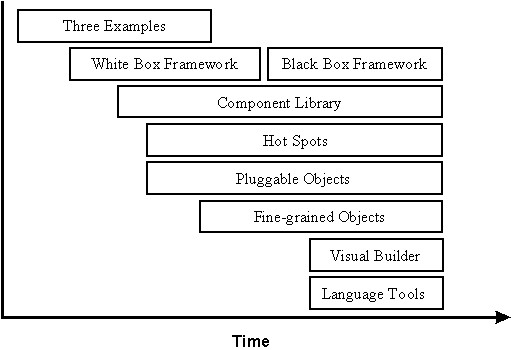
\includegraphics[width=.9\linewidth]{./obrazky-figures/evolving-frameworks.jpg}
\caption{The timeline of patterns as described in Evolving Patterns}
\end{figure}

To briefly describe the terms and how they relate to this work:
\begin{itemize}
\item \textbf{``Three Examples''} are three applications from which the framework will
draw common themes and architecture, so that it fulfills real-world needs. This
is what we will go through in the next section, where we take three existing
application specifications and build a Haskell version of it.
\item In a \textbf{``White Box Framework''}, the architecture is extracted into a separate
library and expanded or re-implemented in further applications. The author
emphasizes 'programming-by-difference', where the programmer extends library
code and later factors out commonly repeated patterns into the library. In
this work, this is the approach taken after implementing the ``Three Examples''
to create the basics of the shared libraries.
\item The next patterns, ``\textbf{Component Library}'', ``\textbf{Hot Spots}'', and
``\textbf{Pluggable/Fine-grained Objects}'' are all an extension of the above, focusing
on extracting concrete components and restructuring the architecture to
improve developer experience in specific ways. This level, nor the further
ones are not implemented in this work.
\item Skipping a ``\textbf{Visual Builder}'', which is not a common pattern in Web frameworks,
there are some basic ``\textbf{Language Tools}'' implemented as a part of creating the
libraries, namely a debugging console for watching specific values and an
inspector of the application storage. [TODO: specify after implementing]
\end{itemize}

Not mentioned as a part of the patterns but also an essential part of framework
development is thorough documentation and guides, as well as test coverage of
library code, which is also done as a part of the work on libraries in the
latter parts of this work.

The above is a quite general description, so we will now enumerate the specifics of the
implementation plan, starting with a reiteration of the requirements of a PWA
from the introduction, which is the end goal of this work.

\begin{itemize}
\item Pages are responsive on tablets \& mobile devices
\item All app URLs load while offline
\item Metadata provided for Add to Home screen
\item Page transitions do not feel like they block on the network
\item Each page has a URL
\item Pages use the History API
\item Site uses cache-first networking
\item Site appropriately informs the user when they are offline
\item Push notifications (consists of several related requirements)
\end{itemize}

There are, however, several components missing in the Haskell ecosystem that
need to be created from scratch:
\begin{itemize}
\item A full-featured browser routing library. While there are some existing
implementations, they are either incomplete or long abandoned.
\item A wrapper around ServiceWorkers, or a template to simplify project creation.
\item A push notifications library. This will need to be both a server-side library,
for creating them, and a client-side consumer, to parse them.
\item A way to prerender the application - either just the HTML ``app shell'' or all
pages on the site.
\item An offline storage library for the client. Here are several possible variants,
in the order of difficulty:
\begin{itemize}
\item plain storage datatype with LocalStorage, SessionStorage, and IndexedDB backends
\item a storage including a transparent cache integrated with the network layer
\item a storage with an invalidation or auto-refresh functionality, using an event
stream from the server
\item a storage with offline-capable synchronization capabilities
\end{itemize}
\end{itemize}

These components do not comprise a fully integrated framework in the sense of
e.g. Angular, such frameworks are quite uncommon in the Haskell ecosystem. More
common are collections of libraries that play well together, where one library
provides the fundamental datatype - the ``architecture'' of the application - and
other libraries fill in the functionality, which is what we will work on. Of the
proposed components, only the routing library is an ``architectural'' one in the
sense that it will influence the shape of the application and its fundamental
data types.

\chapter{Components}
\label{sec:org0d8e10a}
TODO: Demonstrate the principles of components on 'src-snippets' code, where
I will show the smallest possible code that implements that functionality

\section{Component A}
\label{sec:orgc62d9c1}
\subsection{Design}
\label{sec:org91b64af}
\subsection{Implementation}
\label{sec:orgf2038b8}
\subsection{Testing}
\label{sec:org808311a}
\subsection{Other options, possible improvements}
\label{sec:org115cc84}

\chapter{Applications}
\label{sec:orge8a56b4}
\section{Workflow and tools}
\label{sec:org10cd01d}
TODO: describe the development flow of an app built using these tools

\begin{itemize}
\item starting out - three layer cake \& esp. the inner one
\item QA (tests, e2e, CI, \ldots{}), documentation
\item development tool options
\item deployment options
\end{itemize}

\section{TodoMVC}
\label{sec:org16f12be}
There is an abundance of web frameworks, and there are several projects that aim
to give developers a side-by-side comparison of them. Out of these, the original
and most well-known one is TodoMVC \cite{todomvc}, which is aimed at ``MV* frontend
frameworks''. There are currently 64 implementations of their specification -
some of them are variants of the same framework though. There are a few others -
HNPWA is aimed at Progressive Web Applications and it is a tad smaller, with 42
implementations. The last comparison project selected for this work is
RealWorld. This one has both a frontend and a backend part and there is also a
small number of full-stack frameworks. It offers a quite thorough comparison,
with 18 frontends, 34 backends, and 3 full-stack implementations.

We will start with TodoMVC as it is the simplest of the three. TodoMVC is, as
the name hints, a web application for managing a to-do list. It is not a complex
project but it is intended to exercise fundamental features of a framework - DOM
manipulation, forms and validation, state management (in-memory and in
LocalStorage), and routing.

\section{HNPWA}
\label{sec:orga17bf9b}
HNPWA \cite{hnpwa} is a client for Hacker News, a technological news site. Unlike TodoMVC,
HNPWA does not provide a rigid specification and consists only of a rough
guideline of what to implement. The task is to create a Progressive Web
Application that displays information from a given API. The application must be
well optimized (to achieve score 90 in the Lighthouse tool) with optional
server-side rendering.

\section{RealWorld}
\label{sec:org295bddb}
RealWorld \cite{realworld} is the most complex of the comparison projects. It is a clone of
Medium, an online publishing platform, so it requires everything a ``real world''
application would. The task is split into a backend, defined by an API
specification, and a frontend, defined by an HTML structure.

There is a number of features the application needs to support, namely: JWT
(JSON Web Token) authentication with registration and user management, the
ability to post articles and comments, and to follow users and favorite articles.

\chapter{Conclusion}
\label{sec:orgefb0e35}
TODO: return to the comparison with JS, PHP, \ldots{} frameworks

TODO: describe possible follow-up work, what I will be working on - define
specific topics and make concrete examples

-- The final chapter includes an evaluation of the achieved results with a special
emphasis on the student's own contribution. A compulsory assessment of the
project's development will also be required, the student will present ideas
based on the experience with the project and will also show the connections to
the just completed projects. \cite{Pravidla}

% * (bibliography, start of appendix)                           :ignoreheading:
\makeatletter
\def\@openbib@code{\addcontentsline{toc}{chapter}{Bibliography}}
\makeatother
\bibliographystyle{bib-styles/englishiso}

\begin{flushleft}
\bibliography{projekt}
\end{flushleft}
\iftwoside\cleardoublepage\fi

% Appendices
\appendix
\appendixpage
\iftwoside\cleardoublepage\fi

\startcontents[chapters]
% \setlength{\parskip}{0pt}
% \printcontents[chapters]{l}{0}{\setcounter{tocdepth}{2}}
% \setlength{\parskip}{0.5\bigskipamount}
\iftwoside\cleardoublepage\fi

\chapter{Contents of the attached data storage}
\label{sec:org878a2db}
TODO: fill in

\chapter{Poster}
\label{sec:orgd560e1f}
TODO: fill in
\end{document}